\section{Missing matter}

\begin{frame}
    
    \begin{figure}
         \centering
         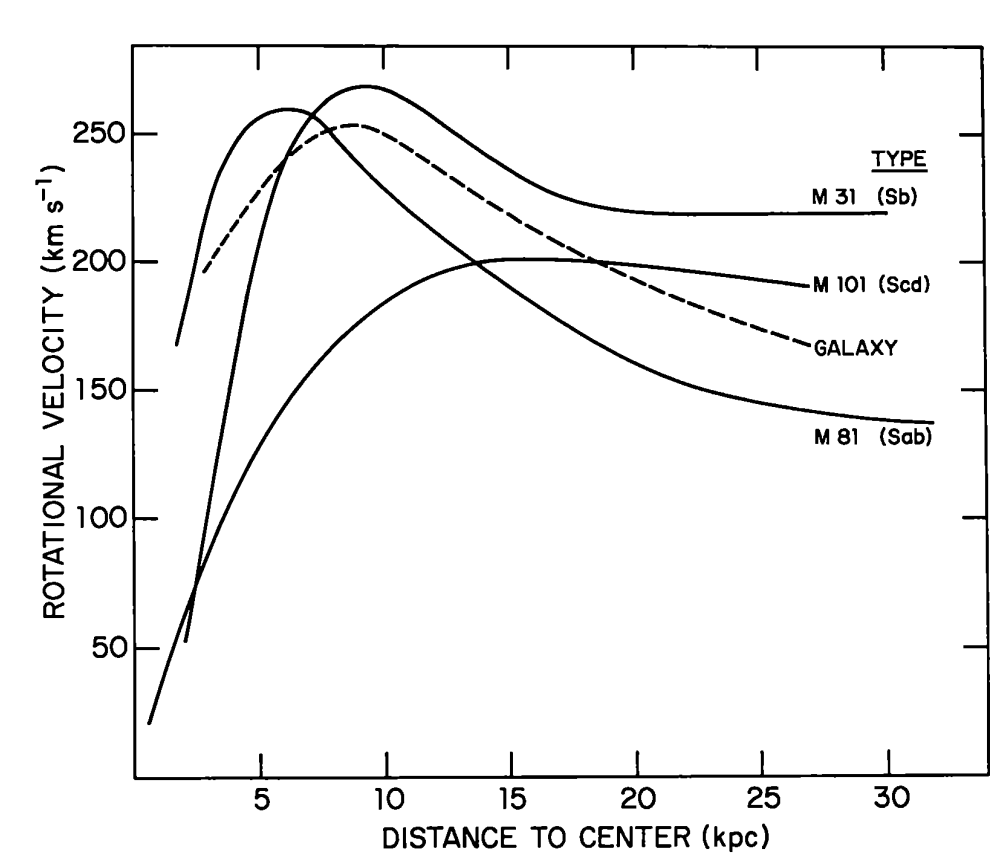
\includegraphics[width=.7\textwidth]{Figures/rotation-curves.png}
        \caption{Rotation curves of some galaxies REFERENCIA}
        \label{fig:rot}
    \end{figure}
    
\end{frame}

\begin{frame}{Models and recipes}
\begin{columns}
\begin{column}{0.5\textwidth}
Properties:
    \begin{itemize}
        \item Neutral
        \item Stable
        \item Cold
        \item Weakly interacting
    \end{itemize}
    \bigskip
Candidates:
    \begin{itemize}
        \item WIMPs
        \item FIMPs
        \item \textcolor{yellow}{Ultralight scalars}
        \textcolor{yellow}{$m_\theta \sim \mathcal{O}(10^{-10}-10^{-20})$ \si{\eV}}
    \end{itemize}
\end{column}
\begin{column}{0.5\textwidth}
Ways to produce:
\begin{itemize}
    \item Freeze-Out
    \item Freeze-In
    \item Cosmic strings
    \item Domain Walls
    \item \textcolor{yellow}{Misalignment mechanism}
\end{itemize}
\end{column}
\end{columns}
\end{frame}